\documentclass[twoside]{book}

% Packages required by doxygen
\usepackage{fixltx2e}
\usepackage{calc}
\usepackage{doxygen}
\usepackage[export]{adjustbox} % also loads graphicx
\usepackage{graphicx}
\usepackage[utf8]{inputenc}
\usepackage{makeidx}
\usepackage{multicol}
\usepackage{multirow}
\PassOptionsToPackage{warn}{textcomp}
\usepackage{textcomp}
\usepackage[nointegrals]{wasysym}
\usepackage[table]{xcolor}

% NLS support packages
\usepackage[brazil]{babel}
% Font selection
\usepackage[T1]{fontenc}
\usepackage[scaled=.90]{helvet}
\usepackage{courier}
\usepackage{amssymb}
\usepackage{sectsty}
\renewcommand{\familydefault}{\sfdefault}
\allsectionsfont{%
  \fontseries{bc}\selectfont%
  \color{darkgray}%
}
\renewcommand{\DoxyLabelFont}{%
  \fontseries{bc}\selectfont%
  \color{darkgray}%
}
\newcommand{\+}{\discretionary{\mbox{\scriptsize$\hookleftarrow$}}{}{}}

% Page & text layout
\usepackage{geometry}
\geometry{%
  a4paper,%
  top=2.5cm,%
  bottom=2.5cm,%
  left=2.5cm,%
  right=2.5cm%
}
\tolerance=750
\hfuzz=15pt
\hbadness=750
\setlength{\emergencystretch}{15pt}
\setlength{\parindent}{0cm}
\setlength{\parskip}{3ex plus 2ex minus 2ex}
\makeatletter
\renewcommand{\paragraph}{%
  \@startsection{paragraph}{4}{0ex}{-1.0ex}{1.0ex}{%
    \normalfont\normalsize\bfseries\SS@parafont%
  }%
}
\renewcommand{\subparagraph}{%
  \@startsection{subparagraph}{5}{0ex}{-1.0ex}{1.0ex}{%
    \normalfont\normalsize\bfseries\SS@subparafont%
  }%
}
\makeatother

% Headers & footers
\usepackage{fancyhdr}
\pagestyle{fancyplain}
\fancyhead[LE]{\fancyplain{}{\bfseries\thepage}}
\fancyhead[CE]{\fancyplain{}{}}
\fancyhead[RE]{\fancyplain{}{\bfseries\leftmark}}
\fancyhead[LO]{\fancyplain{}{\bfseries\rightmark}}
\fancyhead[CO]{\fancyplain{}{}}
\fancyhead[RO]{\fancyplain{}{\bfseries\thepage}}
\fancyfoot[LE]{\fancyplain{}{}}
\fancyfoot[CE]{\fancyplain{}{}}
\fancyfoot[RE]{\fancyplain{}{\bfseries\scriptsize Gerado por Doxygen }}
\fancyfoot[LO]{\fancyplain{}{\bfseries\scriptsize Gerado por Doxygen }}
\fancyfoot[CO]{\fancyplain{}{}}
\fancyfoot[RO]{\fancyplain{}{}}
\renewcommand{\footrulewidth}{0.4pt}
\renewcommand{\chaptermark}[1]{%
  \markboth{#1}{}%
}
\renewcommand{\sectionmark}[1]{%
  \markright{\thesection\ #1}%
}

% Indices & bibliography
\usepackage{natbib}
\usepackage[titles]{tocloft}
\setcounter{tocdepth}{3}
\setcounter{secnumdepth}{5}
\makeindex

% Hyperlinks (required, but should be loaded last)
\usepackage{ifpdf}
\ifpdf
  \usepackage[pdftex,pagebackref=true]{hyperref}
\else
  \usepackage[ps2pdf,pagebackref=true]{hyperref}
\fi
\hypersetup{%
  colorlinks=true,%
  linkcolor=blue,%
  citecolor=blue,%
  unicode%
}

% Custom commands
\newcommand{\clearemptydoublepage}{%
  \newpage{\pagestyle{empty}\cleardoublepage}%
}

\usepackage{caption}
\captionsetup{labelsep=space,justification=centering,font={bf},singlelinecheck=off,skip=4pt,position=top}

%===== C O N T E N T S =====

\begin{document}

% Titlepage & ToC
\hypersetup{pageanchor=false,
             bookmarksnumbered=true,
             pdfencoding=unicode
            }
\pagenumbering{alph}
\begin{titlepage}
\vspace*{7cm}
\begin{center}%
{\Large My Project }\\
\vspace*{1cm}
{\large Gerado por Doxygen 1.8.13}\\
\end{center}
\end{titlepage}
\clearemptydoublepage
\pagenumbering{roman}
\tableofcontents
\clearemptydoublepage
\pagenumbering{arabic}
\hypersetup{pageanchor=true}

%--- Begin generated contents ---
\chapter{Índice dos Componentes}
\section{Lista de Componentes}
Aqui estão as classes, estruturas, uniões e interfaces e suas respectivas descrições\+:\begin{DoxyCompactList}
\item\contentsline{section}{\hyperlink{classSculptor}{Sculptor} }{\pageref{classSculptor}}{}
\item\contentsline{section}{\hyperlink{structVoxel}{Voxel} }{\pageref{structVoxel}}{}
\end{DoxyCompactList}

\chapter{Índice dos Arquivos}
\section{Lista de Arquivos}
Esta é a lista de todos os arquivos e suas respectivas descrições\+:\begin{DoxyCompactList}
\item\contentsline{section}{\hyperlink{main_8cpp}{main.\+cpp} }{\pageref{main_8cpp}}{}
\item\contentsline{section}{\hyperlink{Sculptor_8cpp}{Sculptor.\+cpp} }{\pageref{Sculptor_8cpp}}{}
\item\contentsline{section}{\hyperlink{Sculptor_8h}{Sculptor.\+h} }{\pageref{Sculptor_8h}}{}
\end{DoxyCompactList}

\chapter{Classes}
\hypertarget{classSculptor}{}\section{Referência da Classe Sculptor}
\label{classSculptor}\index{Sculptor@{Sculptor}}


{\ttfamily \#include $<$Sculptor.\+h$>$}



Diagrama de colaboração para Sculptor\+:\nopagebreak
\begin{figure}[H]
\begin{center}
\leavevmode
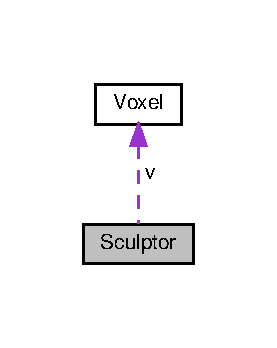
\includegraphics[width=133pt]{classSculptor__coll__graph}
\end{center}
\end{figure}
\subsection*{Métodos Públicos}
\begin{DoxyCompactItemize}
\item 
\hyperlink{classSculptor_a014e3ef5517bf0e9d9e14486b6ac6433}{Sculptor} (int \+\_\+nx, int \+\_\+ny, int \+\_\+nz)
\begin{DoxyCompactList}\small\item\em Construtor da classe. \end{DoxyCompactList}\item 
\hyperlink{classSculptor_a8f159bf97458326f16d2e238e11be7ff}{$\sim$\+Sculptor} ()
\item 
void \hyperlink{classSculptor_a4e53f85ee03b729efafa985f72563c4b}{set\+Color} (float \+\_\+r, float \+\_\+g, float \+\_\+b, float alpha)
\item 
void \hyperlink{classSculptor_a4bdea3048b419d58e93074060eaa7b52}{put\+Voxel} (int x, int y, int z)
\item 
void \hyperlink{classSculptor_ad9d714a35fc8ae16d06eb5df37c3493c}{cut\+Voxel} (int x, int y, int z)
\item 
void \hyperlink{classSculptor_a311ad7a0fb83fc67ac1f378be8e99fe1}{put\+Box} (int x0, int x1, int y0, int y1, int z0, int z1)
\item 
void \hyperlink{classSculptor_aa84a1b12b09e9e103fc8d78f8d1bc00f}{cut\+Box} (int x0, int x1, int y0, int y1, int z0, int z1)
\item 
void \hyperlink{classSculptor_a794a2b6ee8fc8098fd6150cb46101fc6}{put\+Sphere} (int xcenter, int ycenter, int zcenter, int radius)
\item 
void \hyperlink{classSculptor_a67ab8c0ba5116adb8af1d01ad373ac15}{cut\+Sphere} (int xcenter, int ycenter, int zcenter, int radius)
\item 
void \hyperlink{classSculptor_a093615b0c2b9b3a17a56300b9b939f39}{put\+Ellipsoid} (int xcenter, int ycenter, int zcenter, int rx, int ry, int rz)
\item 
void \hyperlink{classSculptor_a18d2922c111c4c13653ee07d878151ad}{cut\+Ellipsoid} (int xcenter, int ycenter, int zcenter, int rx, int ry, int rz)
\item 
void \hyperlink{classSculptor_aa8ed61fc7cae10c4d7a895330fe5e309}{write\+O\+FF} (char $\ast$filename)
\end{DoxyCompactItemize}
\subsection*{Atributos Públicos}
\begin{DoxyCompactItemize}
\item 
int \hyperlink{classSculptor_a9ec05cea70fece563fa9fdea340696db}{numE}
\end{DoxyCompactItemize}
\subsection*{Atributos Protegidos}
\begin{DoxyCompactItemize}
\item 
int \hyperlink{classSculptor_ad1e32f9042538419a3bc7b376f7813b8}{nx}
\item 
int \hyperlink{classSculptor_a1ce2ff97ec94927928ab3f5ec4ba6761}{ny}
\item 
int \hyperlink{classSculptor_a33204e7df26a7ee4c7192381a24335d3}{nz}
\item 
float \hyperlink{classSculptor_a3f5d2ec3b66d645019b8d81c810a1cd8}{r}
\item 
float \hyperlink{classSculptor_a208c06af69a81a1568df4493868816f1}{g}
\item 
float \hyperlink{classSculptor_a7aafd7305ea634252d8288b60536cd96}{b}
\item 
float \hyperlink{classSculptor_a6fd0157dcf17582f0edd5fddf157604e}{a}
\item 
\hyperlink{structVoxel}{Voxel} $\ast$$\ast$$\ast$ \hyperlink{classSculptor_a4ca53a2f2fbf41ca42dfe729ebe693f1}{v}
\end{DoxyCompactItemize}


\subsection{Construtores \& Destrutores}
\mbox{\Hypertarget{classSculptor_a014e3ef5517bf0e9d9e14486b6ac6433}\label{classSculptor_a014e3ef5517bf0e9d9e14486b6ac6433}} 
\index{Sculptor@{Sculptor}!Sculptor@{Sculptor}}
\index{Sculptor@{Sculptor}!Sculptor@{Sculptor}}
\subsubsection{\texorpdfstring{Sculptor()}{Sculptor()}}
{\footnotesize\ttfamily Sculptor\+::\+Sculptor (\begin{DoxyParamCaption}\item[{int}]{\+\_\+nx,  }\item[{int}]{\+\_\+ny,  }\item[{int}]{\+\_\+nz }\end{DoxyParamCaption})}



Construtor da classe. 

$<$ faço V apontar para zero para ter um parametro que a alocação da memória ocorreu de forma correta

$<$ seta os valores das dimensões do espaço 3D

$<$ chamada da função para alocação da memória necesária \mbox{\Hypertarget{classSculptor_a8f159bf97458326f16d2e238e11be7ff}\label{classSculptor_a8f159bf97458326f16d2e238e11be7ff}} 
\index{Sculptor@{Sculptor}!````~Sculptor@{$\sim$\+Sculptor}}
\index{````~Sculptor@{$\sim$\+Sculptor}!Sculptor@{Sculptor}}
\subsubsection{\texorpdfstring{$\sim$\+Sculptor()}{~Sculptor()}}
{\footnotesize\ttfamily Sculptor\+::$\sim$\+Sculptor (\begin{DoxyParamCaption}{ }\end{DoxyParamCaption})}

$<$ Libera o espaço da memória antes usado para guardar o espaço de 3D do objeto

$<$ dessa forma posso reutilizar o ponteiro 

\subsection{Métodos}
\mbox{\Hypertarget{classSculptor_aa84a1b12b09e9e103fc8d78f8d1bc00f}\label{classSculptor_aa84a1b12b09e9e103fc8d78f8d1bc00f}} 
\index{Sculptor@{Sculptor}!cut\+Box@{cut\+Box}}
\index{cut\+Box@{cut\+Box}!Sculptor@{Sculptor}}
\subsubsection{\texorpdfstring{cut\+Box()}{cutBox()}}
{\footnotesize\ttfamily void Sculptor\+::cut\+Box (\begin{DoxyParamCaption}\item[{int}]{x0,  }\item[{int}]{x1,  }\item[{int}]{y0,  }\item[{int}]{y1,  }\item[{int}]{z0,  }\item[{int}]{z1 }\end{DoxyParamCaption})}

\mbox{\Hypertarget{classSculptor_a18d2922c111c4c13653ee07d878151ad}\label{classSculptor_a18d2922c111c4c13653ee07d878151ad}} 
\index{Sculptor@{Sculptor}!cut\+Ellipsoid@{cut\+Ellipsoid}}
\index{cut\+Ellipsoid@{cut\+Ellipsoid}!Sculptor@{Sculptor}}
\subsubsection{\texorpdfstring{cut\+Ellipsoid()}{cutEllipsoid()}}
{\footnotesize\ttfamily void Sculptor\+::cut\+Ellipsoid (\begin{DoxyParamCaption}\item[{int}]{xcenter,  }\item[{int}]{ycenter,  }\item[{int}]{zcenter,  }\item[{int}]{rx,  }\item[{int}]{ry,  }\item[{int}]{rz }\end{DoxyParamCaption})}

$<$ verifica se o pixel satisfaz a equação da esfera com os parametros informados \mbox{\Hypertarget{classSculptor_a67ab8c0ba5116adb8af1d01ad373ac15}\label{classSculptor_a67ab8c0ba5116adb8af1d01ad373ac15}} 
\index{Sculptor@{Sculptor}!cut\+Sphere@{cut\+Sphere}}
\index{cut\+Sphere@{cut\+Sphere}!Sculptor@{Sculptor}}
\subsubsection{\texorpdfstring{cut\+Sphere()}{cutSphere()}}
{\footnotesize\ttfamily void Sculptor\+::cut\+Sphere (\begin{DoxyParamCaption}\item[{int}]{xcenter,  }\item[{int}]{ycenter,  }\item[{int}]{zcenter,  }\item[{int}]{radius }\end{DoxyParamCaption})}

$<$ verifica se o pixel satisfaz a equação da esfera com os parametros informados \mbox{\Hypertarget{classSculptor_ad9d714a35fc8ae16d06eb5df37c3493c}\label{classSculptor_ad9d714a35fc8ae16d06eb5df37c3493c}} 
\index{Sculptor@{Sculptor}!cut\+Voxel@{cut\+Voxel}}
\index{cut\+Voxel@{cut\+Voxel}!Sculptor@{Sculptor}}
\subsubsection{\texorpdfstring{cut\+Voxel()}{cutVoxel()}}
{\footnotesize\ttfamily void Sculptor\+::cut\+Voxel (\begin{DoxyParamCaption}\item[{int}]{x,  }\item[{int}]{y,  }\item[{int}]{z }\end{DoxyParamCaption})}

\mbox{\Hypertarget{classSculptor_a311ad7a0fb83fc67ac1f378be8e99fe1}\label{classSculptor_a311ad7a0fb83fc67ac1f378be8e99fe1}} 
\index{Sculptor@{Sculptor}!put\+Box@{put\+Box}}
\index{put\+Box@{put\+Box}!Sculptor@{Sculptor}}
\subsubsection{\texorpdfstring{put\+Box()}{putBox()}}
{\footnotesize\ttfamily void Sculptor\+::put\+Box (\begin{DoxyParamCaption}\item[{int}]{x0,  }\item[{int}]{x1,  }\item[{int}]{y0,  }\item[{int}]{y1,  }\item[{int}]{z0,  }\item[{int}]{z1 }\end{DoxyParamCaption})}

\mbox{\Hypertarget{classSculptor_a093615b0c2b9b3a17a56300b9b939f39}\label{classSculptor_a093615b0c2b9b3a17a56300b9b939f39}} 
\index{Sculptor@{Sculptor}!put\+Ellipsoid@{put\+Ellipsoid}}
\index{put\+Ellipsoid@{put\+Ellipsoid}!Sculptor@{Sculptor}}
\subsubsection{\texorpdfstring{put\+Ellipsoid()}{putEllipsoid()}}
{\footnotesize\ttfamily void Sculptor\+::put\+Ellipsoid (\begin{DoxyParamCaption}\item[{int}]{xcenter,  }\item[{int}]{ycenter,  }\item[{int}]{zcenter,  }\item[{int}]{rx,  }\item[{int}]{ry,  }\item[{int}]{rz }\end{DoxyParamCaption})}

$<$ verifica se o pixel satisfaz a equação da esfera com os parametros informados \mbox{\Hypertarget{classSculptor_a794a2b6ee8fc8098fd6150cb46101fc6}\label{classSculptor_a794a2b6ee8fc8098fd6150cb46101fc6}} 
\index{Sculptor@{Sculptor}!put\+Sphere@{put\+Sphere}}
\index{put\+Sphere@{put\+Sphere}!Sculptor@{Sculptor}}
\subsubsection{\texorpdfstring{put\+Sphere()}{putSphere()}}
{\footnotesize\ttfamily void Sculptor\+::put\+Sphere (\begin{DoxyParamCaption}\item[{int}]{xcenter,  }\item[{int}]{ycenter,  }\item[{int}]{zcenter,  }\item[{int}]{radius }\end{DoxyParamCaption})}

$<$ verifica se o pixel satisfaz a equação da esfera com os parametros informados \mbox{\Hypertarget{classSculptor_a4bdea3048b419d58e93074060eaa7b52}\label{classSculptor_a4bdea3048b419d58e93074060eaa7b52}} 
\index{Sculptor@{Sculptor}!put\+Voxel@{put\+Voxel}}
\index{put\+Voxel@{put\+Voxel}!Sculptor@{Sculptor}}
\subsubsection{\texorpdfstring{put\+Voxel()}{putVoxel()}}
{\footnotesize\ttfamily void Sculptor\+::put\+Voxel (\begin{DoxyParamCaption}\item[{int}]{x,  }\item[{int}]{y,  }\item[{int}]{z }\end{DoxyParamCaption})}

\mbox{\Hypertarget{classSculptor_a4e53f85ee03b729efafa985f72563c4b}\label{classSculptor_a4e53f85ee03b729efafa985f72563c4b}} 
\index{Sculptor@{Sculptor}!set\+Color@{set\+Color}}
\index{set\+Color@{set\+Color}!Sculptor@{Sculptor}}
\subsubsection{\texorpdfstring{set\+Color()}{setColor()}}
{\footnotesize\ttfamily void Sculptor\+::set\+Color (\begin{DoxyParamCaption}\item[{float}]{\+\_\+r,  }\item[{float}]{\+\_\+g,  }\item[{float}]{\+\_\+b,  }\item[{float}]{alpha }\end{DoxyParamCaption})}

$<$ seta os valores da cores a serem usadas \mbox{\Hypertarget{classSculptor_aa8ed61fc7cae10c4d7a895330fe5e309}\label{classSculptor_aa8ed61fc7cae10c4d7a895330fe5e309}} 
\index{Sculptor@{Sculptor}!write\+O\+FF@{write\+O\+FF}}
\index{write\+O\+FF@{write\+O\+FF}!Sculptor@{Sculptor}}
\subsubsection{\texorpdfstring{write\+O\+F\+F()}{writeOFF()}}
{\footnotesize\ttfamily void Sculptor\+::write\+O\+FF (\begin{DoxyParamCaption}\item[{char $\ast$}]{filename }\end{DoxyParamCaption})}

cria o arquivo .O\+FF

$<$ testar

escreve a primeira linha do arquivo .O\+FF

$<$ P0

$<$ P1

$<$ P2

$<$ P3

$<$ P4

$<$ P5

$<$ P6

$<$ P7

$<$ face 1

$<$ face 2

$<$ face 3

$<$ face 4

$<$ face 5

$<$ face 6 

\subsection{Atributos}
\mbox{\Hypertarget{classSculptor_a6fd0157dcf17582f0edd5fddf157604e}\label{classSculptor_a6fd0157dcf17582f0edd5fddf157604e}} 
\index{Sculptor@{Sculptor}!a@{a}}
\index{a@{a}!Sculptor@{Sculptor}}
\subsubsection{\texorpdfstring{a}{a}}
{\footnotesize\ttfamily float Sculptor\+::a\hspace{0.3cm}{\ttfamily [protected]}}

\mbox{\Hypertarget{classSculptor_a7aafd7305ea634252d8288b60536cd96}\label{classSculptor_a7aafd7305ea634252d8288b60536cd96}} 
\index{Sculptor@{Sculptor}!b@{b}}
\index{b@{b}!Sculptor@{Sculptor}}
\subsubsection{\texorpdfstring{b}{b}}
{\footnotesize\ttfamily float Sculptor\+::b\hspace{0.3cm}{\ttfamily [protected]}}

\mbox{\Hypertarget{classSculptor_a208c06af69a81a1568df4493868816f1}\label{classSculptor_a208c06af69a81a1568df4493868816f1}} 
\index{Sculptor@{Sculptor}!g@{g}}
\index{g@{g}!Sculptor@{Sculptor}}
\subsubsection{\texorpdfstring{g}{g}}
{\footnotesize\ttfamily float Sculptor\+::g\hspace{0.3cm}{\ttfamily [protected]}}

\mbox{\Hypertarget{classSculptor_a9ec05cea70fece563fa9fdea340696db}\label{classSculptor_a9ec05cea70fece563fa9fdea340696db}} 
\index{Sculptor@{Sculptor}!numE@{numE}}
\index{numE@{numE}!Sculptor@{Sculptor}}
\subsubsection{\texorpdfstring{numE}{numE}}
{\footnotesize\ttfamily int Sculptor\+::numE}

\mbox{\Hypertarget{classSculptor_ad1e32f9042538419a3bc7b376f7813b8}\label{classSculptor_ad1e32f9042538419a3bc7b376f7813b8}} 
\index{Sculptor@{Sculptor}!nx@{nx}}
\index{nx@{nx}!Sculptor@{Sculptor}}
\subsubsection{\texorpdfstring{nx}{nx}}
{\footnotesize\ttfamily int Sculptor\+::nx\hspace{0.3cm}{\ttfamily [protected]}}

\mbox{\Hypertarget{classSculptor_a1ce2ff97ec94927928ab3f5ec4ba6761}\label{classSculptor_a1ce2ff97ec94927928ab3f5ec4ba6761}} 
\index{Sculptor@{Sculptor}!ny@{ny}}
\index{ny@{ny}!Sculptor@{Sculptor}}
\subsubsection{\texorpdfstring{ny}{ny}}
{\footnotesize\ttfamily int Sculptor\+::ny\hspace{0.3cm}{\ttfamily [protected]}}

\mbox{\Hypertarget{classSculptor_a33204e7df26a7ee4c7192381a24335d3}\label{classSculptor_a33204e7df26a7ee4c7192381a24335d3}} 
\index{Sculptor@{Sculptor}!nz@{nz}}
\index{nz@{nz}!Sculptor@{Sculptor}}
\subsubsection{\texorpdfstring{nz}{nz}}
{\footnotesize\ttfamily int Sculptor\+::nz\hspace{0.3cm}{\ttfamily [protected]}}

\mbox{\Hypertarget{classSculptor_a3f5d2ec3b66d645019b8d81c810a1cd8}\label{classSculptor_a3f5d2ec3b66d645019b8d81c810a1cd8}} 
\index{Sculptor@{Sculptor}!r@{r}}
\index{r@{r}!Sculptor@{Sculptor}}
\subsubsection{\texorpdfstring{r}{r}}
{\footnotesize\ttfamily float Sculptor\+::r\hspace{0.3cm}{\ttfamily [protected]}}

\mbox{\Hypertarget{classSculptor_a4ca53a2f2fbf41ca42dfe729ebe693f1}\label{classSculptor_a4ca53a2f2fbf41ca42dfe729ebe693f1}} 
\index{Sculptor@{Sculptor}!v@{v}}
\index{v@{v}!Sculptor@{Sculptor}}
\subsubsection{\texorpdfstring{v}{v}}
{\footnotesize\ttfamily \hyperlink{structVoxel}{Voxel}$\ast$$\ast$$\ast$ Sculptor\+::v\hspace{0.3cm}{\ttfamily [protected]}}



A documentação para esta classe foi gerada a partir dos seguintes arquivos\+:\begin{DoxyCompactItemize}
\item 
\hyperlink{Sculptor_8h}{Sculptor.\+h}\item 
\hyperlink{Sculptor_8cpp}{Sculptor.\+cpp}\end{DoxyCompactItemize}

\hypertarget{structVoxel}{}\section{Referência da Estrutura Voxel}
\label{structVoxel}\index{Voxel@{Voxel}}


{\ttfamily \#include $<$Sculptor.\+h$>$}

\subsection*{Atributos Públicos}
\begin{DoxyCompactItemize}
\item 
float \hyperlink{structVoxel_a06872ec79b836120b551a848968c0f1b}{r}
\item 
float \hyperlink{structVoxel_a27c0da1ed2ff430401d23ff171612a73}{g}
\item 
float \hyperlink{structVoxel_a5cd8432b1d7d0fd8b79e0fc7d10373a8}{b}
\item 
float \hyperlink{structVoxel_a3ce2579eb0a9f09a07112ce7498a638e}{a}
\item 
bool \hyperlink{structVoxel_a6fbe8bd53f64685ac4210726d40fc775}{is\+On}
\end{DoxyCompactItemize}


\subsection{Atributos}
\mbox{\Hypertarget{structVoxel_a3ce2579eb0a9f09a07112ce7498a638e}\label{structVoxel_a3ce2579eb0a9f09a07112ce7498a638e}} 
\index{Voxel@{Voxel}!a@{a}}
\index{a@{a}!Voxel@{Voxel}}
\subsubsection{\texorpdfstring{a}{a}}
{\footnotesize\ttfamily float Voxel\+::a}

\mbox{\Hypertarget{structVoxel_a5cd8432b1d7d0fd8b79e0fc7d10373a8}\label{structVoxel_a5cd8432b1d7d0fd8b79e0fc7d10373a8}} 
\index{Voxel@{Voxel}!b@{b}}
\index{b@{b}!Voxel@{Voxel}}
\subsubsection{\texorpdfstring{b}{b}}
{\footnotesize\ttfamily float Voxel\+::b}

\mbox{\Hypertarget{structVoxel_a27c0da1ed2ff430401d23ff171612a73}\label{structVoxel_a27c0da1ed2ff430401d23ff171612a73}} 
\index{Voxel@{Voxel}!g@{g}}
\index{g@{g}!Voxel@{Voxel}}
\subsubsection{\texorpdfstring{g}{g}}
{\footnotesize\ttfamily float Voxel\+::g}

\mbox{\Hypertarget{structVoxel_a6fbe8bd53f64685ac4210726d40fc775}\label{structVoxel_a6fbe8bd53f64685ac4210726d40fc775}} 
\index{Voxel@{Voxel}!is\+On@{is\+On}}
\index{is\+On@{is\+On}!Voxel@{Voxel}}
\subsubsection{\texorpdfstring{is\+On}{isOn}}
{\footnotesize\ttfamily bool Voxel\+::is\+On}

\mbox{\Hypertarget{structVoxel_a06872ec79b836120b551a848968c0f1b}\label{structVoxel_a06872ec79b836120b551a848968c0f1b}} 
\index{Voxel@{Voxel}!r@{r}}
\index{r@{r}!Voxel@{Voxel}}
\subsubsection{\texorpdfstring{r}{r}}
{\footnotesize\ttfamily float Voxel\+::r}



A documentação para esta estrutura foi gerada a partir do seguinte arquivo\+:\begin{DoxyCompactItemize}
\item 
\hyperlink{Sculptor_8h}{Sculptor.\+h}\end{DoxyCompactItemize}

\chapter{Arquivos}
\hypertarget{main_8cpp}{}\section{Referência do Arquivo main.\+cpp}
\label{main_8cpp}\index{main.\+cpp@{main.\+cpp}}
{\ttfamily \#include $<$iostream$>$}\newline
{\ttfamily \#include $<$Sculptor.\+h$>$}\newline
{\ttfamily \#include $<$string$>$}\newline
Gráfico de dependência de inclusões para main.\+cpp\+:\nopagebreak
\begin{figure}[H]
\begin{center}
\leavevmode
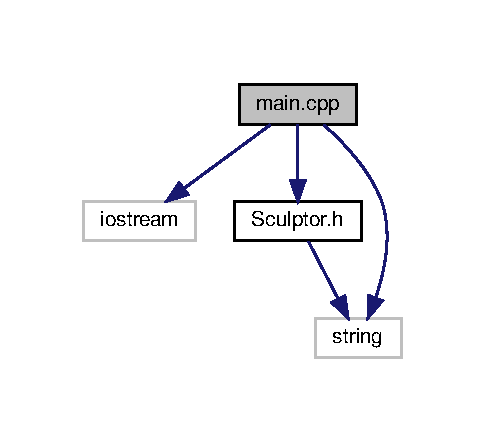
\includegraphics[width=233pt]{main_8cpp__incl}
\end{center}
\end{figure}
\subsection*{Funções}
\begin{DoxyCompactItemize}
\item 
int \hyperlink{main_8cpp_ae66f6b31b5ad750f1fe042a706a4e3d4}{main} ()
\end{DoxyCompactItemize}
\subsection*{Variáveis}
\begin{DoxyCompactItemize}
\item 
char $\ast$ \hyperlink{main_8cpp_aebbb100c552614c2fdb3a2d4bc3260c7}{Teste\+Esculptor} = \char`\"{}Escultura\char`\"{}
\end{DoxyCompactItemize}


\subsection{Funções}
\mbox{\Hypertarget{main_8cpp_ae66f6b31b5ad750f1fe042a706a4e3d4}\label{main_8cpp_ae66f6b31b5ad750f1fe042a706a4e3d4}} 
\index{main.\+cpp@{main.\+cpp}!main@{main}}
\index{main@{main}!main.\+cpp@{main.\+cpp}}
\subsubsection{\texorpdfstring{main()}{main()}}
{\footnotesize\ttfamily int main (\begin{DoxyParamCaption}{ }\end{DoxyParamCaption})}



\subsection{Variáveis}
\mbox{\Hypertarget{main_8cpp_aebbb100c552614c2fdb3a2d4bc3260c7}\label{main_8cpp_aebbb100c552614c2fdb3a2d4bc3260c7}} 
\index{main.\+cpp@{main.\+cpp}!Teste\+Esculptor@{Teste\+Esculptor}}
\index{Teste\+Esculptor@{Teste\+Esculptor}!main.\+cpp@{main.\+cpp}}
\subsubsection{\texorpdfstring{Teste\+Esculptor}{TesteEsculptor}}
{\footnotesize\ttfamily char$\ast$ Teste\+Esculptor = \char`\"{}Escultura\char`\"{}}


\hypertarget{Sculptor_8cpp}{}\section{Referência do Arquivo Sculptor.\+cpp}
\label{Sculptor_8cpp}\index{Sculptor.\+cpp@{Sculptor.\+cpp}}
{\ttfamily \#include $<$iostream$>$}\newline
{\ttfamily \#include $<$fstream$>$}\newline
{\ttfamily \#include $<$Sculptor.\+h$>$}\newline
Gráfico de dependência de inclusões para Sculptor.\+cpp\+:\nopagebreak
\begin{figure}[H]
\begin{center}
\leavevmode
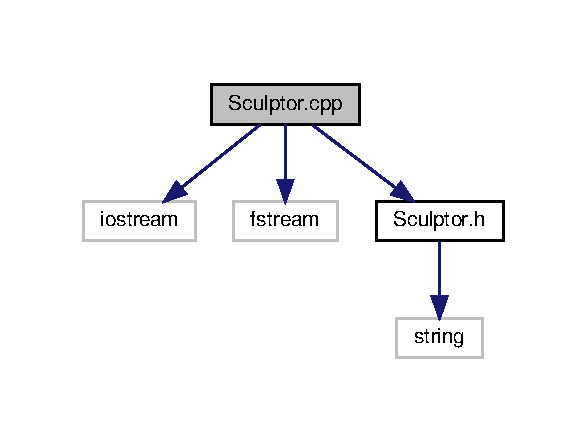
\includegraphics[width=282pt]{Sculptor_8cpp__incl}
\end{center}
\end{figure}
\subsection*{Funções}
\begin{DoxyCompactItemize}
\item 
\hyperlink{structVoxel}{Voxel} $\ast$$\ast$$\ast$ \hyperlink{Sculptor_8cpp_a702174f787dbf131405d9ddccb240611}{aloca\+Espaco} (int nc, int na, int nl)
\item 
bool \hyperlink{Sculptor_8cpp_a038fe43a962d4018b69218cd036b947a}{verifica\+Cord} (int x, int y, int z, int nc, int na, int nl)
\item 
bool \hyperlink{Sculptor_8cpp_aabf9cc6b6b14c65c22f065d37ae46114}{satisfaz\+Eq\+Esfera} (int z, int x, int y, int a, int b, int c, int raio)
\item 
bool \hyperlink{Sculptor_8cpp_af3991c70607baa62e160b3e034cc6340}{satisfaz\+Eq\+Elipse} (int z, int x, int y, int xcent, int ycent, int zcent, int a, int b, int c)
\end{DoxyCompactItemize}


\subsection{Funções}
\mbox{\Hypertarget{Sculptor_8cpp_a702174f787dbf131405d9ddccb240611}\label{Sculptor_8cpp_a702174f787dbf131405d9ddccb240611}} 
\index{Sculptor.\+cpp@{Sculptor.\+cpp}!aloca\+Espaco@{aloca\+Espaco}}
\index{aloca\+Espaco@{aloca\+Espaco}!Sculptor.\+cpp@{Sculptor.\+cpp}}
\subsubsection{\texorpdfstring{aloca\+Espaco()}{alocaEspaco()}}
{\footnotesize\ttfamily \hyperlink{structVoxel}{Voxel}$\ast$$\ast$$\ast$ aloca\+Espaco (\begin{DoxyParamCaption}\item[{int}]{nc,  }\item[{int}]{na,  }\item[{int}]{nl }\end{DoxyParamCaption})}

Fução aloca\+Espaco

função \char`\"{}aloca\+Espaco\char`\"{} tem esse nome devido a sua função do escultor,  é responsável por alocar o espaço tridimensional onde ser feito a escultura 3D  é feita uma alocação de uma matriz, onde cada elemento dessa matriz recebe  vetor que corresponde a altura desse espaço.

alocação referente as linhas da matriz

$<$ verifica se a alocação da memória foi feita da forma correta

alocação das colunas de forma onde o primeiro endereço de \char`\"{}aux\char`\"{} contenha o primeiro endereço referente ao vetor de colunas da minha matriz. A iteração que vem logo em seguida serve para ajustar os endereços de memoria de forma que fiquem sequenciais

$<$ Iteração para ajuste das posições do eixo X na memória \mbox{\Hypertarget{Sculptor_8cpp_af3991c70607baa62e160b3e034cc6340}\label{Sculptor_8cpp_af3991c70607baa62e160b3e034cc6340}} 
\index{Sculptor.\+cpp@{Sculptor.\+cpp}!satisfaz\+Eq\+Elipse@{satisfaz\+Eq\+Elipse}}
\index{satisfaz\+Eq\+Elipse@{satisfaz\+Eq\+Elipse}!Sculptor.\+cpp@{Sculptor.\+cpp}}
\subsubsection{\texorpdfstring{satisfaz\+Eq\+Elipse()}{satisfazEqElipse()}}
{\footnotesize\ttfamily bool satisfaz\+Eq\+Elipse (\begin{DoxyParamCaption}\item[{int}]{z,  }\item[{int}]{x,  }\item[{int}]{y,  }\item[{int}]{xcent,  }\item[{int}]{ycent,  }\item[{int}]{zcent,  }\item[{int}]{a,  }\item[{int}]{b,  }\item[{int}]{c }\end{DoxyParamCaption})}

\mbox{\Hypertarget{Sculptor_8cpp_aabf9cc6b6b14c65c22f065d37ae46114}\label{Sculptor_8cpp_aabf9cc6b6b14c65c22f065d37ae46114}} 
\index{Sculptor.\+cpp@{Sculptor.\+cpp}!satisfaz\+Eq\+Esfera@{satisfaz\+Eq\+Esfera}}
\index{satisfaz\+Eq\+Esfera@{satisfaz\+Eq\+Esfera}!Sculptor.\+cpp@{Sculptor.\+cpp}}
\subsubsection{\texorpdfstring{satisfaz\+Eq\+Esfera()}{satisfazEqEsfera()}}
{\footnotesize\ttfamily bool satisfaz\+Eq\+Esfera (\begin{DoxyParamCaption}\item[{int}]{z,  }\item[{int}]{x,  }\item[{int}]{y,  }\item[{int}]{a,  }\item[{int}]{b,  }\item[{int}]{c,  }\item[{int}]{raio }\end{DoxyParamCaption})}

\mbox{\Hypertarget{Sculptor_8cpp_a038fe43a962d4018b69218cd036b947a}\label{Sculptor_8cpp_a038fe43a962d4018b69218cd036b947a}} 
\index{Sculptor.\+cpp@{Sculptor.\+cpp}!verifica\+Cord@{verifica\+Cord}}
\index{verifica\+Cord@{verifica\+Cord}!Sculptor.\+cpp@{Sculptor.\+cpp}}
\subsubsection{\texorpdfstring{verifica\+Cord()}{verificaCord()}}
{\footnotesize\ttfamily bool verifica\+Cord (\begin{DoxyParamCaption}\item[{int}]{x,  }\item[{int}]{y,  }\item[{int}]{z,  }\item[{int}]{nc,  }\item[{int}]{na,  }\item[{int}]{nl }\end{DoxyParamCaption})}

função para averiguar se as coordenadas passadas como parametro pertencem ao espaço tridimencional com tamanho informado (x,y,z) são as coordenadas que seram verificadas (nc,na,nl) são as dimensões do espaço 3D que será usado, correspondentes a (nx,ny,nz) respectivamente 
\hypertarget{Sculptor_8h}{}\section{Referência do Arquivo Sculptor.\+h}
\label{Sculptor_8h}\index{Sculptor.\+h@{Sculptor.\+h}}
{\ttfamily \#include $<$string$>$}\newline
Gráfico de dependência de inclusões para Sculptor.\+h\+:\nopagebreak
\begin{figure}[H]
\begin{center}
\leavevmode
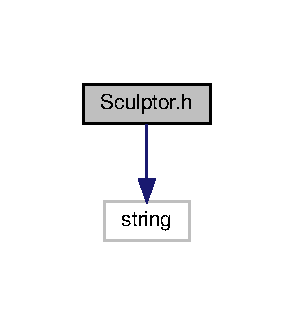
\includegraphics[width=141pt]{Sculptor_8h__incl}
\end{center}
\end{figure}
Este grafo mostra quais arquivos estão direta ou indiretamente relacionados com este arquivo\+:\nopagebreak
\begin{figure}[H]
\begin{center}
\leavevmode
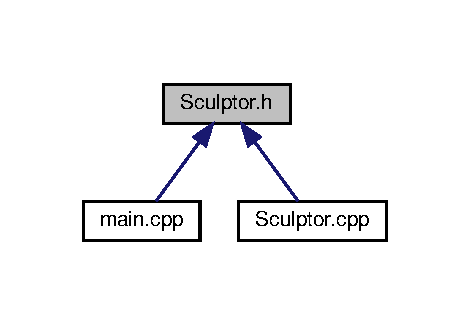
\includegraphics[width=226pt]{Sculptor_8h__dep__incl}
\end{center}
\end{figure}
\subsection*{Componentes}
\begin{DoxyCompactItemize}
\item 
struct \hyperlink{structVoxel}{Voxel}
\item 
class \hyperlink{classSculptor}{Sculptor}
\end{DoxyCompactItemize}

%--- End generated contents ---

% Index
\backmatter
\newpage
\phantomsection
\clearemptydoublepage
\addcontentsline{toc}{chapter}{Índice}
\printindex

\end{document}
